%!TEX root = thesis.tex

% Singel glacier test cases
\chapter{Single glacier test cases}\label{appendix_A}
\thispagestyle{plain}

The first experiment was performend as a single glacier test case on the example of Hintereisferner (RGI60-11.00897), see Section~\ref{sub:experimental_setup_test_case} for details on the experimental setup. The test case was intended to get a first qualitative impression, drawing conclusions from a single data point is, however, still questionable. Therefore, the exact same experiment was performend on five more single glaciers (Pasterze, Mer de Glace, Glacier d'Argentière, Großer Aletschgletscher, Rhonegletscher) and the results are shown here below. While there are differences between the different glaciers, all general findings presented in Section~\ref{sub:results_test_case} hold true.

\begin{figure}[p]
  \centering

  % VAS volume
  \begin{subfigure}[b]{0.476\textwidth}
    \caption{\Vas{} model, relative ice volume}
    \label{fig:Pasterze:volume_vas}
    \centering
    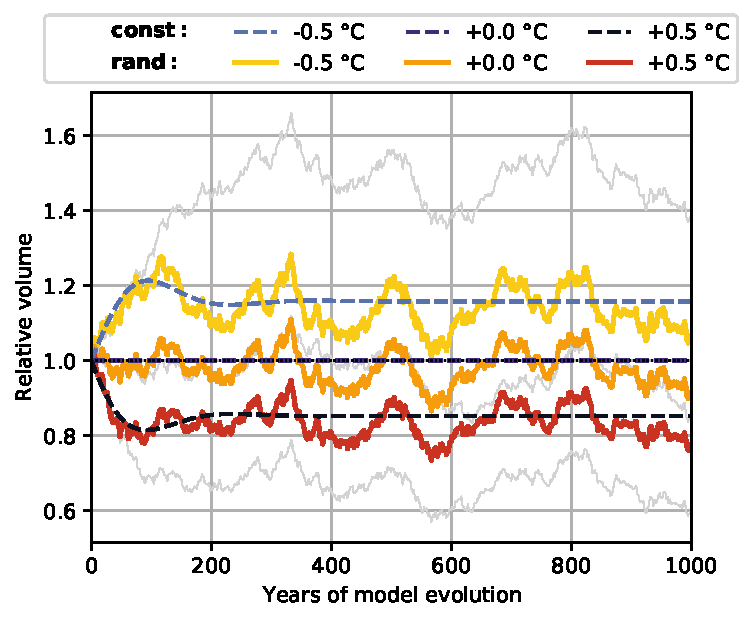
\includegraphics[width=\textwidth]{../plots/final_plots/time_series/single_glaciers/volume_norm_vas_Pasterze.pdf}
  \end{subfigure}
  \hfill
  % Flowline volume
  \begin{subfigure}[b]{0.476\textwidth}
    \caption{Flowline model, relative ice volume}
    \label{fig:Pasterze:volume_fl}
    \centering
    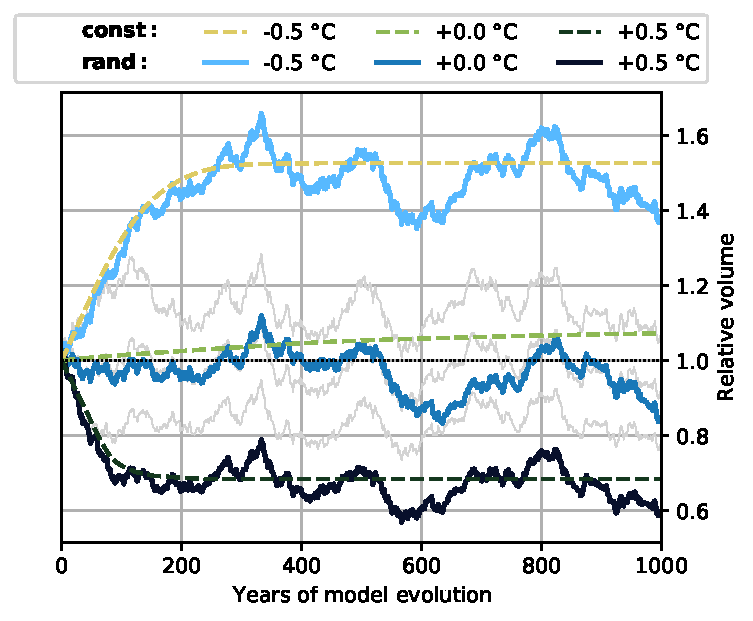
\includegraphics[width=\textwidth]{../plots/final_plots/time_series/single_glaciers/volume_norm_fl_Pasterze.pdf}
  \end{subfigure}

  % VAS area
  \begin{subfigure}[b]{0.476\textwidth}
    \caption{\Vas{} model, relative surface area}
    \label{fig:Pasterze:area_vas}
    \centering
    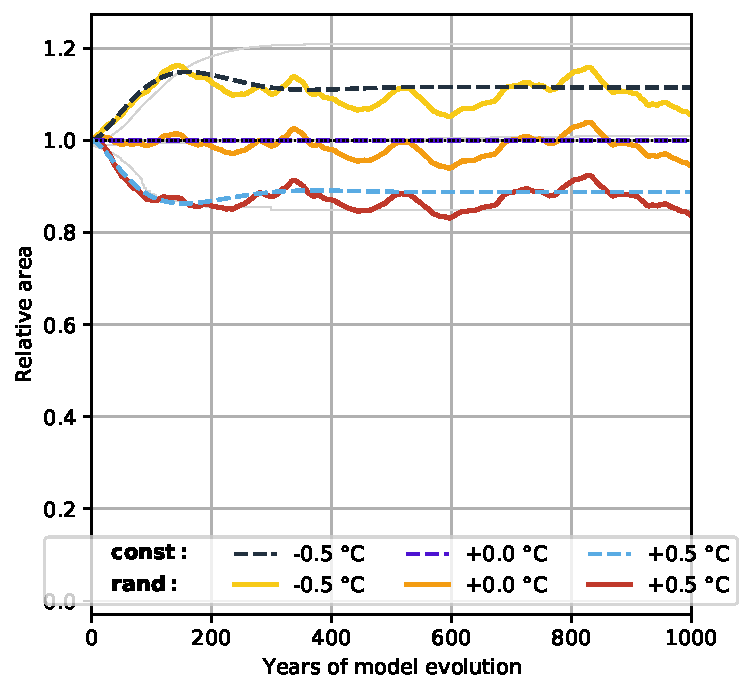
\includegraphics[width=\textwidth]{../plots/final_plots/time_series/single_glaciers/area_norm_vas_Pasterze.pdf}
  \end{subfigure}
  \hfill
  % Flowline area
  \begin{subfigure}[b]{0.476\textwidth}
    \caption{Flowline model, relative surface area}
    \label{fig:Pasterze:area_fl}
    \centering
    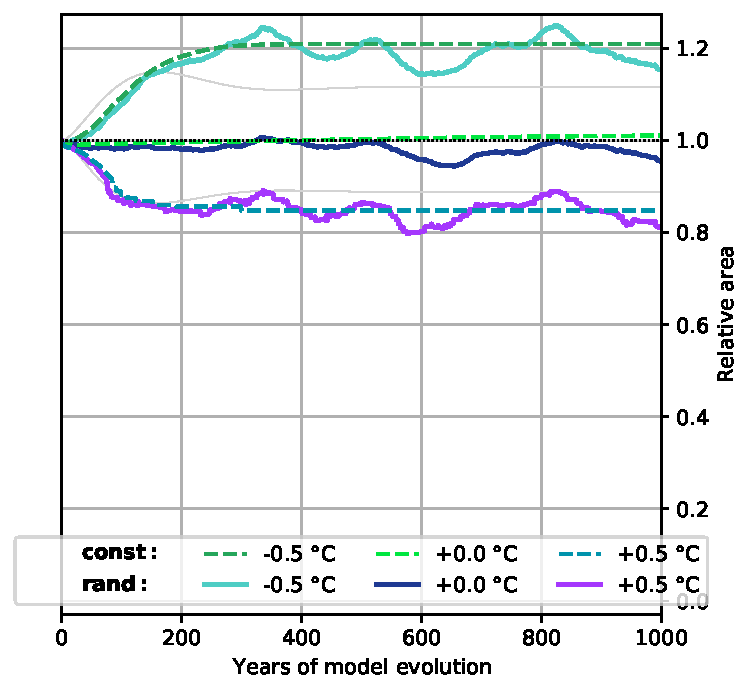
\includegraphics[width=\textwidth]{../plots/final_plots/time_series/single_glaciers/area_norm_fl_Pasterze.pdf}
  \end{subfigure}

  % VAS length
  \begin{subfigure}[b]{0.476\textwidth}
    \caption{\Vas{} model, relative glacier length}
    \label{fig:Pasterze:length_vas}
    \centering
    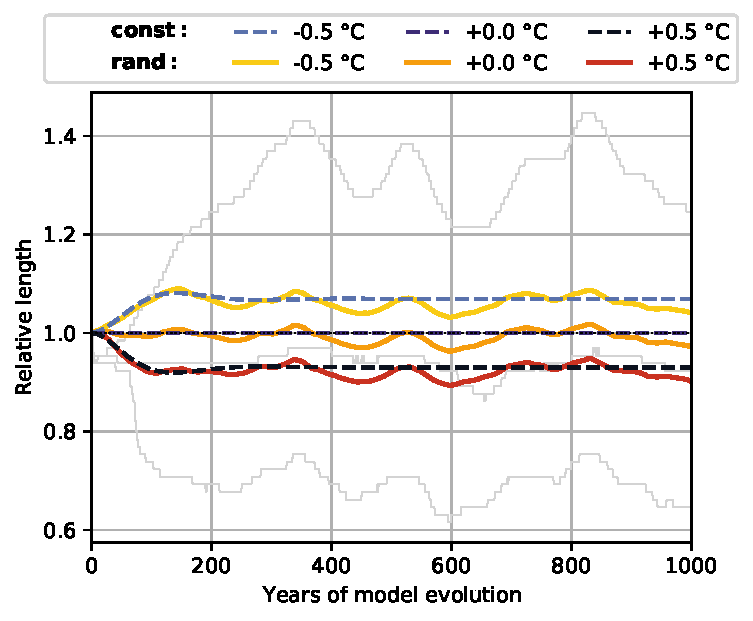
\includegraphics[width=\textwidth]{../plots/final_plots/time_series/single_glaciers/length_norm_vas_Pasterze.pdf}
  \end{subfigure}
  \hfill
  % Flowline length
  \begin{subfigure}[b]{0.476\textwidth}
    \caption{Flowline model, relative glacier length}
    \label{fig:Pasterze:length_fl}
    \centering
    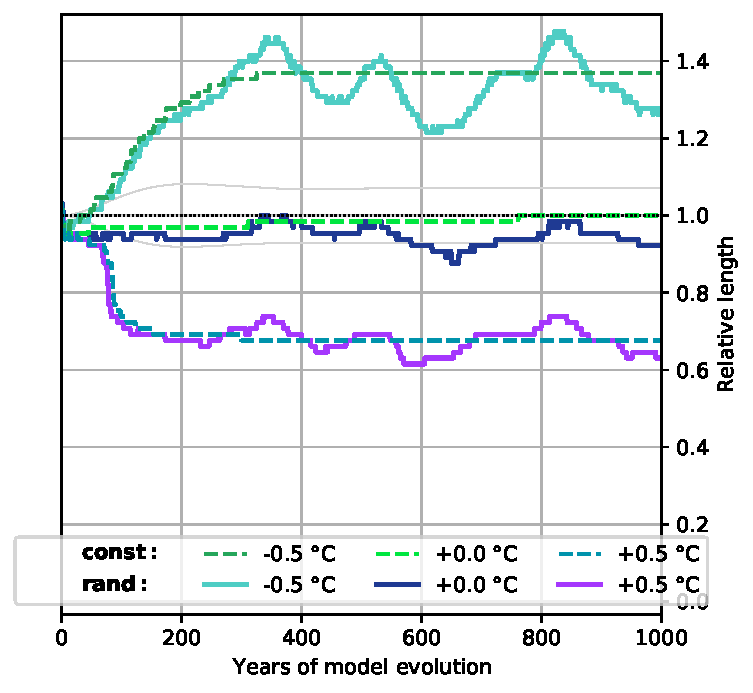
\includegraphics[width=\textwidth]{../plots/final_plots/time_series/single_glaciers/length_norm_fl_Pasterze.pdf}
  \end{subfigure}
  
  \caption{Temporal evolution of ice volume in (\subref{fig:Pasterze:volume_vas}) and (\subref{fig:Pasterze:volume_fl}), surface area in (\subref{fig:Pasterze:area_vas}) and (\subref{fig:Pasterze:area_fl}) and glacier length in (\subref{fig:Pasterze:length_vas}) and (\subref{fig:Pasterze:length_fl}) for \textbf{Pasterze (RGI60-11.00106)}. The shown values area normalized with their respective initial values. The left panels show the result of the \vas{} model, the right panels show the results of the flowline model. Solid lines represent the random climate scenarios, while dashed lines represent the constant climate scenarios. All climate scenarios are based on an equilibrium climate. The applied temperature biases of \SI{-.5}{\celsius}, \SI{0}{\celsius} and \SI{+.5}{\celsius} are color coded, see legend for details. The dotted line indicates the initial volume. The light gray lines represent the volume evolutions of the other model, to facilitate comparisons.}
  \label{fig:Pasterze}
\end{figure}

\begin{figure}[p]
  \centering

  % VAS volume
  \begin{subfigure}[b]{0.476\textwidth}
    \caption{\Vas{} model, relative ice volume}
    \label{fig:Mer_de_Glace:volume_vas}
    \centering
    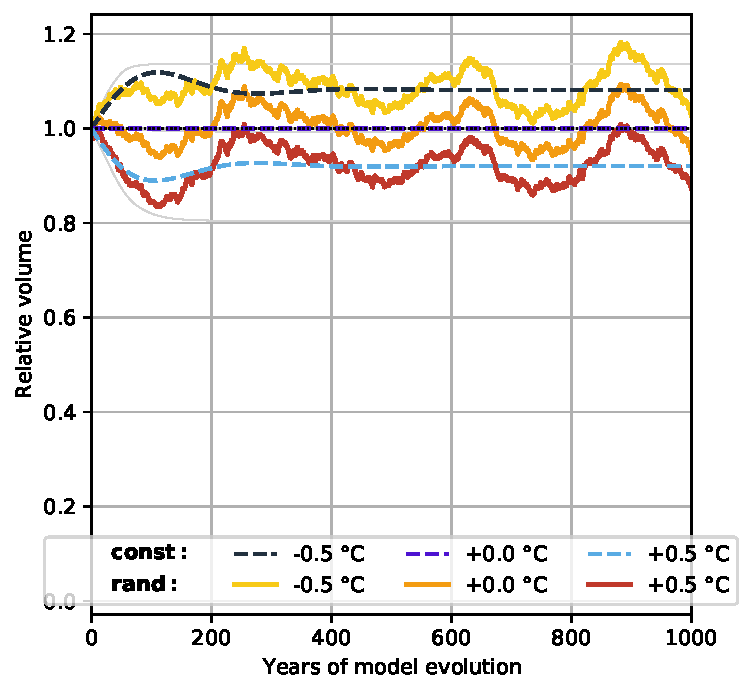
\includegraphics[width=\textwidth]{../plots/final_plots/time_series/single_glaciers/volume_norm_vas_Mer_de_Glace.pdf}
  \end{subfigure}
  \hfill
  % Flowline volume
  \begin{subfigure}[b]{0.476\textwidth}
    \caption{Flowline model, relative ice volume}
    \label{fig:Mer_de_Glace:volume_fl}
    \centering
    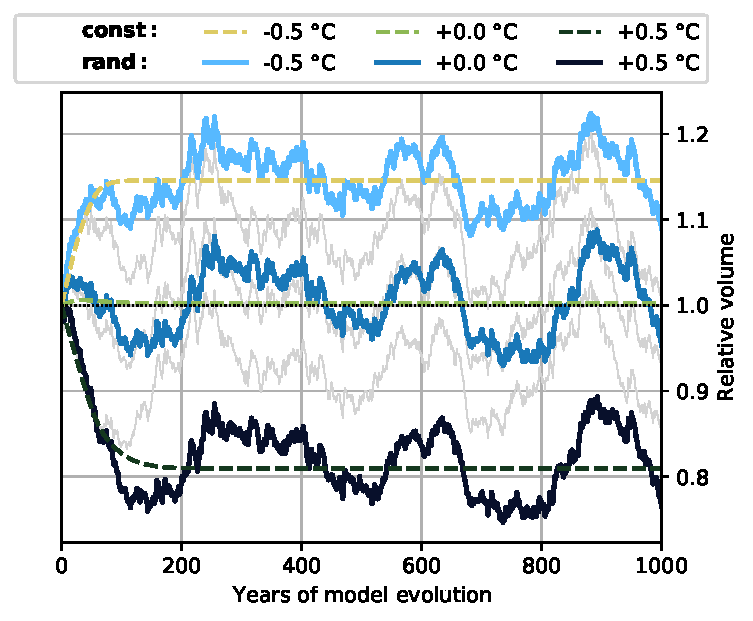
\includegraphics[width=\textwidth]{../plots/final_plots/time_series/single_glaciers/volume_norm_fl_Mer_de_Glace.pdf}
  \end{subfigure}

  % VAS area
  \begin{subfigure}[b]{0.476\textwidth}
    \caption{\Vas{} model, relative surface area}
    \label{fig:Mer_de_Glace:area_vas}
    \centering
    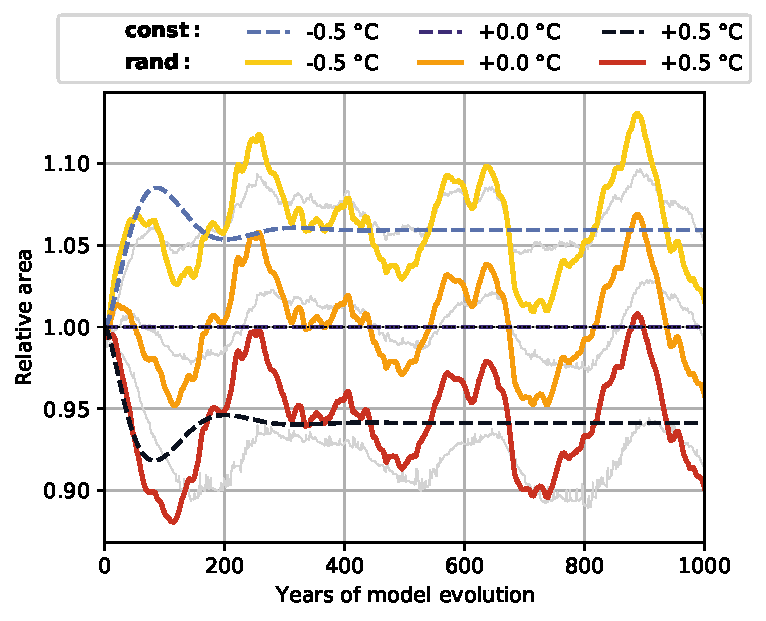
\includegraphics[width=\textwidth]{../plots/final_plots/time_series/single_glaciers/area_norm_vas_Mer_de_Glace.pdf}
  \end{subfigure}
  \hfill
  % Flowline area
  \begin{subfigure}[b]{0.476\textwidth}
    \caption{Flowline model, relative surface area}
    \label{fig:Mer_de_Glace:area_fl}
    \centering
    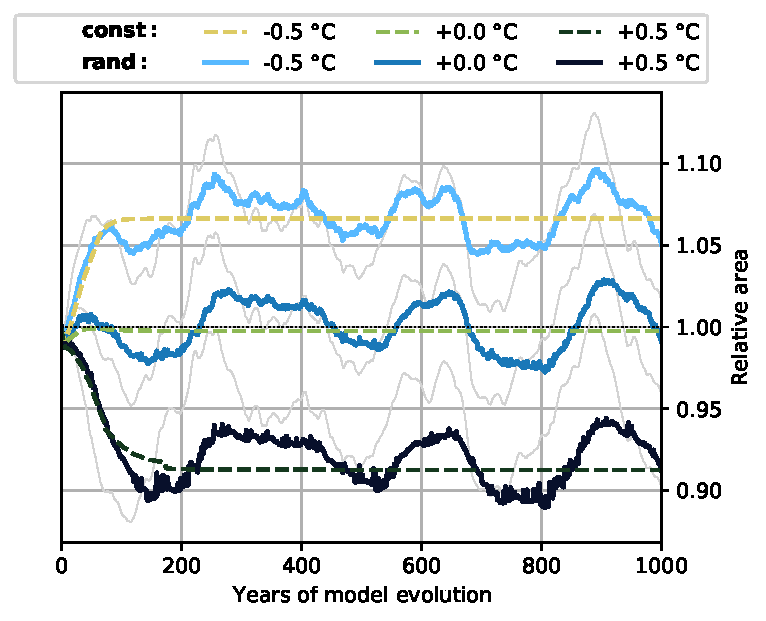
\includegraphics[width=\textwidth]{../plots/final_plots/time_series/single_glaciers/area_norm_fl_Mer_de_Glace.pdf}
  \end{subfigure}

  % VAS length
  \begin{subfigure}[b]{0.476\textwidth}
    \caption{\Vas{} model, relative glacier length}
    \label{fig:Mer_de_Glace:length_vas}
    \centering
    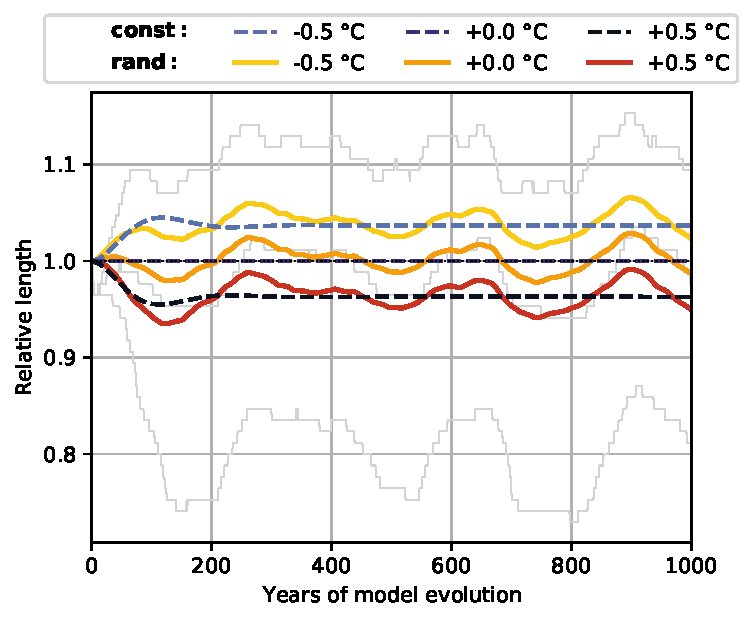
\includegraphics[width=\textwidth]{../plots/final_plots/time_series/single_glaciers/length_norm_vas_Mer_de_Glace.pdf}
  \end{subfigure}
  \hfill
  % Flowline length
  \begin{subfigure}[b]{0.476\textwidth}
    \caption{Flowline model, relative glacier length}
    \label{fig:Mer_de_Glace:length_fl}
    \centering
    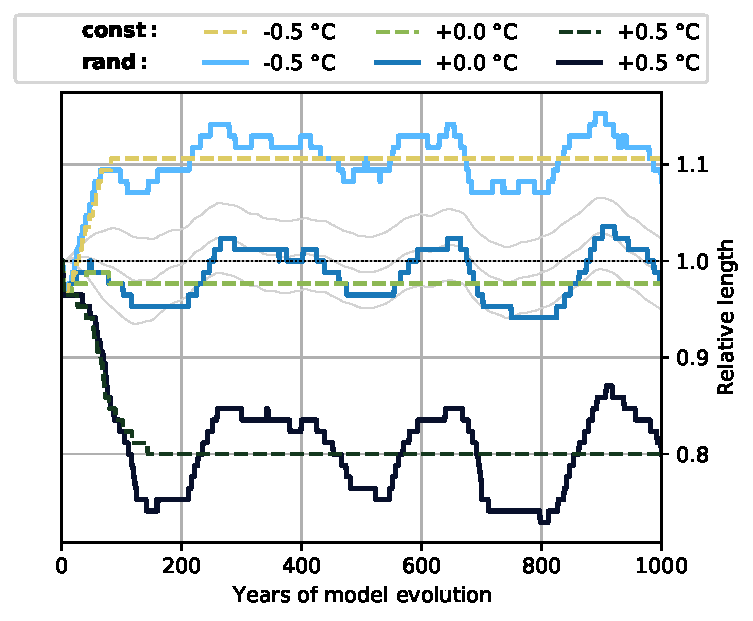
\includegraphics[width=\textwidth]{../plots/final_plots/time_series/single_glaciers/length_norm_fl_Mer_de_Glace.pdf}
  \end{subfigure}
  
  \caption{Temporal evolution of ice volume in (\subref{fig:Mer_de_Glace:volume_vas}) and (\subref{fig:Mer_de_Glace:volume_fl}), surface area in (\subref{fig:Mer_de_Glace:area_vas}) and (\subref{fig:Mer_de_Glace:area_fl}) and glacier length in (\subref{fig:Mer_de_Glace:length_vas}) and (\subref{fig:Mer_de_Glace:length_fl}) for \textbf{Mer de Glace (RGI60-11.03643)}. The shown values area normalized with their respective initial values. The left panels show the result of the \vas{} model, the right panels show the results of the flowline model. Solid lines represent the random climate scenarios, while dashed lines represent the constant climate scenarios. All climate scenarios are based on an equilibrium climate. The applied temperature biases of \SI{-.5}{\celsius}, \SI{0}{\celsius} and \SI{+.5}{\celsius} are color coded, see legend for details. The dotted line indicates the initial volume. The light gray lines represent the volume evolutions of the other model, to facilitate comparisons.}
  \label{fig:Mer_de_Glace}
\end{figure}

\begin{figure}[p]
  \centering

  % VAS volume
  \begin{subfigure}[b]{0.476\textwidth}
    \caption{\Vas{} model, relative ice volume}
    \label{fig:Glacier_d_Argentiere:volume_vas}
    \centering
    \includegraphics[width=\textwidth]{../plots/final_plots/time_series/single_glaciers/volume_norm_vas_Glacier_d'Argentière.pdf}
  \end{subfigure}
  \hfill
  % Flowline volume
  \begin{subfigure}[b]{0.476\textwidth}
    \caption{Flowline model, relative ice volume}
    \label{fig:Glacier_d_Argentiere:volume_fl}
    \centering
    \includegraphics[width=\textwidth]{../plots/final_plots/time_series/single_glaciers/volume_norm_fl_Glacier_d'Argentière.pdf}
  \end{subfigure}

  % VAS area
  \begin{subfigure}[b]{0.476\textwidth}
    \caption{\Vas{} model, relative surface area}
    \label{fig:Glacier_d_Argentiere:area_vas}
    \centering
    \includegraphics[width=\textwidth]{../plots/final_plots/time_series/single_glaciers/area_norm_vas_Glacier_d'Argentière.pdf}
  \end{subfigure}
  \hfill
  % Flowline area
  \begin{subfigure}[b]{0.476\textwidth}
    \caption{Flowline model, relative surface area}
    \label{fig:Glacier_d_Argentiere:area_fl}
    \centering
    \includegraphics[width=\textwidth]{../plots/final_plots/time_series/single_glaciers/area_norm_fl_Glacier_d'Argentière.pdf}
  \end{subfigure}

  % VAS length
  \begin{subfigure}[b]{0.476\textwidth}
    \caption{\Vas{} model, relative glacier length}
    \label{fig:Glacier_d_Argentiere:length_vas}
    \centering
    \includegraphics[width=\textwidth]{../plots/final_plots/time_series/single_glaciers/length_norm_vas_Glacier_d'Argentière.pdf}
  \end{subfigure}
  \hfill
  % Flowline length
  \begin{subfigure}[b]{0.476\textwidth}
    \caption{Flowline model, relative glacier length}
    \label{fig:Glacier_d_Argentiere:length_fl}
    \centering
    \includegraphics[width=\textwidth]{../plots/final_plots/time_series/single_glaciers/length_norm_fl_Glacier_d'Argentière.pdf}
  \end{subfigure}
  
  \caption{Temporal evolution of ice volume in (\subref{fig:Glacier_d_Argentiere:volume_vas}) and (\subref{fig:Glacier_d_Argentiere:volume_fl}), surface area in (\subref{fig:Glacier_d_Argentiere:area_vas}) and (\subref{fig:Glacier_d_Argentiere:area_fl}) and glacier length in (\subref{fig:Glacier_d_Argentiere:length_vas}) and (\subref{fig:Glacier_d_Argentiere:length_fl}) for \textbf{Glacier d'Argentière (RGI60-11.03638)}. The shown values area normalized with their respective initial values. The left panels show the result of the \vas{} model, the right panels show the results of the flowline model. Solid lines represent the random climate scenarios, while dashed lines represent the constant climate scenarios. All climate scenarios are based on an equilibrium climate. The applied temperature biases of \SI{-.5}{\celsius}, \SI{0}{\celsius} and \SI{+.5}{\celsius} are color coded, see legend for details. The dotted line indicates the initial volume. The light gray lines represent the volume evolutions of the other model, to facilitate comparisons.}
  \label{fig:Glacier_d_Argentiere}
\end{figure}

\begin{figure}[p]
  \centering

  % VAS volume
  \begin{subfigure}[b]{0.476\textwidth}
    \caption{\Vas{} model, relative ice volume}
    \label{fig:Grosser_Aletschgletscher:volume_vas}
    \centering
    \includegraphics[width=\textwidth]{../plots/final_plots/time_series/single_glaciers/volume_norm_vas_Großer_Aletschgletscher.pdf}
  \end{subfigure}
  \hfill
  % Flowline volume
  \begin{subfigure}[b]{0.476\textwidth}
    \caption{Flowline model, relative ice volume}
    \label{fig:Grosser_Aletschgletscher:volume_fl}
    \centering
    \includegraphics[width=\textwidth]{../plots/final_plots/time_series/single_glaciers/volume_norm_fl_Großer_Aletschgletscher.pdf}
  \end{subfigure}

  % VAS area
  \begin{subfigure}[b]{0.476\textwidth}
    \caption{\Vas{} model, relative surface area}
    \label{fig:Grosser_Aletschgletscher:area_vas}
    \centering
    \includegraphics[width=\textwidth]{../plots/final_plots/time_series/single_glaciers/area_norm_vas_Großer_Aletschgletscher.pdf}
  \end{subfigure}
  \hfill
  % Flowline area
  \begin{subfigure}[b]{0.476\textwidth}
    \caption{Flowline model, relative surface area}
    \label{fig:Grosser_Aletschgletscher:area_fl}
    \centering
    \includegraphics[width=\textwidth]{../plots/final_plots/time_series/single_glaciers/area_norm_fl_Großer_Aletschgletscher.pdf}
  \end{subfigure}

  % VAS length
  \begin{subfigure}[b]{0.476\textwidth}
    \caption{\Vas{} model, relative glacier length}
    \label{fig:Grosser_Aletschgletscher:length_vas}
    \centering
    \includegraphics[width=\textwidth]{../plots/final_plots/time_series/single_glaciers/length_norm_vas_Großer_Aletschgletscher.pdf}
  \end{subfigure}
  \hfill
  % Flowline length
  \begin{subfigure}[b]{0.476\textwidth}
    \caption{Flowline model, relative glacier length}
    \label{fig:Grosser_Aletschgletscher:length_fl}
    \centering
    \includegraphics[width=\textwidth]{../plots/final_plots/time_series/single_glaciers/length_norm_fl_Großer_Aletschgletscher.pdf}
  \end{subfigure}
  
  \caption{Temporal evolution of ice volume in (\subref{fig:Grosser_Aletschgletscher:volume_vas}) and (\subref{fig:Grosser_Aletschgletscher:volume_fl}), surface area in (\subref{fig:Grosser_Aletschgletscher:area_vas}) and (\subref{fig:Grosser_Aletschgletscher:area_fl}) and glacier length in (\subref{fig:Grosser_Aletschgletscher:length_vas}) and (\subref{fig:Grosser_Aletschgletscher:length_fl}) for \textbf{Großer Aletschgletscher (RGI60-11.01450)}. The shown values area normalized with their respective initial values. The left panels show the result of the \vas{} model, the right panels show the results of the flowline model. Solid lines represent the random climate scenarios, while dashed lines represent the constant climate scenarios. All climate scenarios are based on an equilibrium climate. The applied temperature biases of \SI{-.5}{\celsius}, \SI{0}{\celsius} and \SI{+.5}{\celsius} are color coded, see legend for details. The dotted line indicates the initial volume. The light gray lines represent the volume evolutions of the other model, to facilitate comparisons.}
  \label{fig:Grosser_Aletschgletscher}
\end{figure}

\begin{figure}[p]
  \centering

  % VAS volume
  \begin{subfigure}[b]{0.476\textwidth}
    \caption{\Vas{} model, relative ice volume}
    \label{fig:Rhonegletscher:volume_vas}
    \centering
    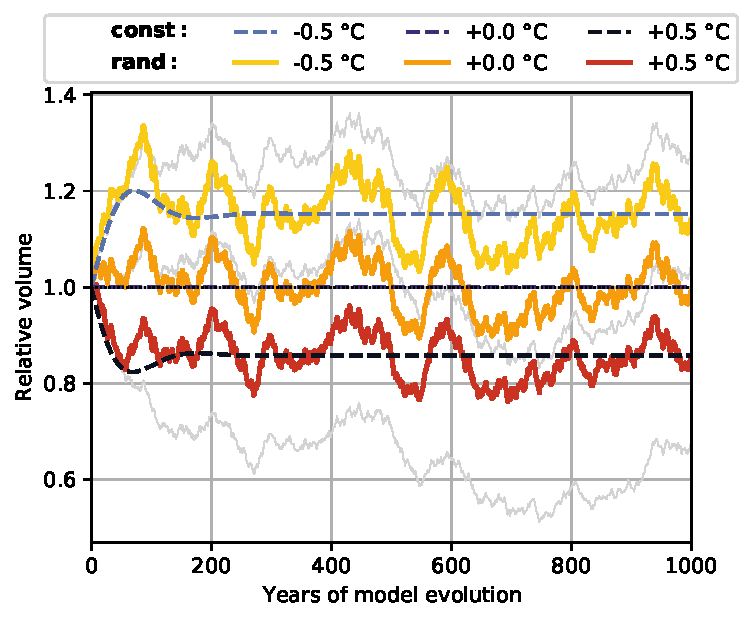
\includegraphics[width=\textwidth]{../plots/final_plots/time_series/single_glaciers/volume_norm_vas_Rhonegletscher.pdf}
  \end{subfigure}
  \hfill
  % Flowline volume
  \begin{subfigure}[b]{0.476\textwidth}
    \caption{Flowline model, relative ice volume}
    \label{fig:Rhonegletscher:volume_fl}
    \centering
    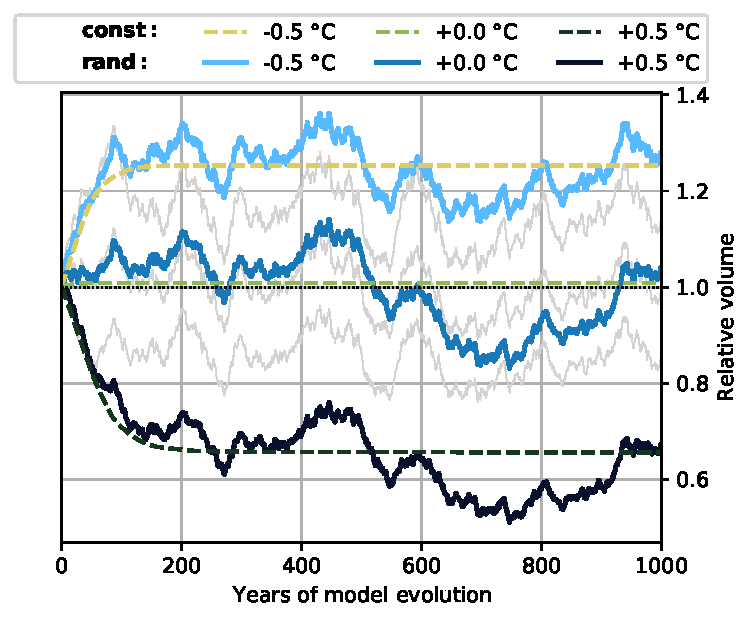
\includegraphics[width=\textwidth]{../plots/final_plots/time_series/single_glaciers/volume_norm_fl_Rhonegletscher.pdf}
  \end{subfigure}

  % VAS area
  \begin{subfigure}[b]{0.476\textwidth}
    \caption{\Vas{} model, relative surface area}
    \label{fig:Rhonegletscher:area_vas}
    \centering
    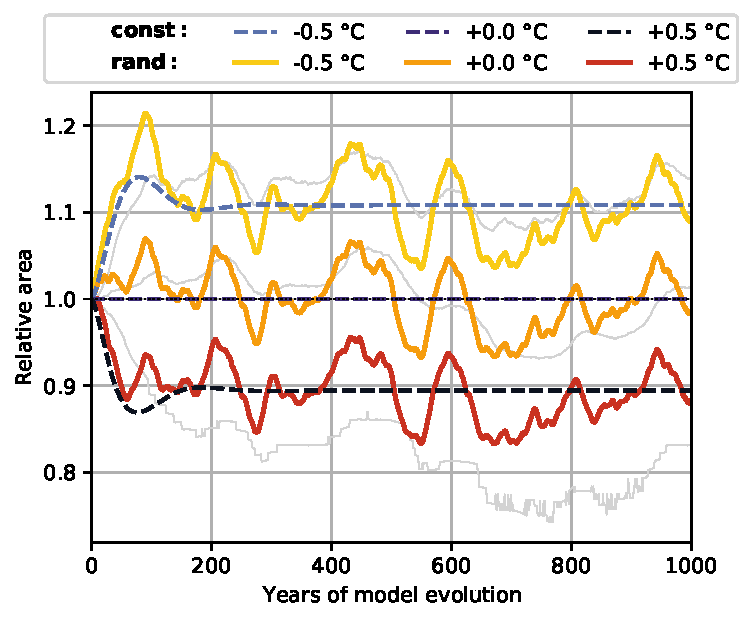
\includegraphics[width=\textwidth]{../plots/final_plots/time_series/single_glaciers/area_norm_vas_Rhonegletscher.pdf}
  \end{subfigure}
  \hfill
  % Flowline area
  \begin{subfigure}[b]{0.476\textwidth}
    \caption{Flowline model, relative surface area}
    \label{fig:Rhonegletscher:area_fl}
    \centering
    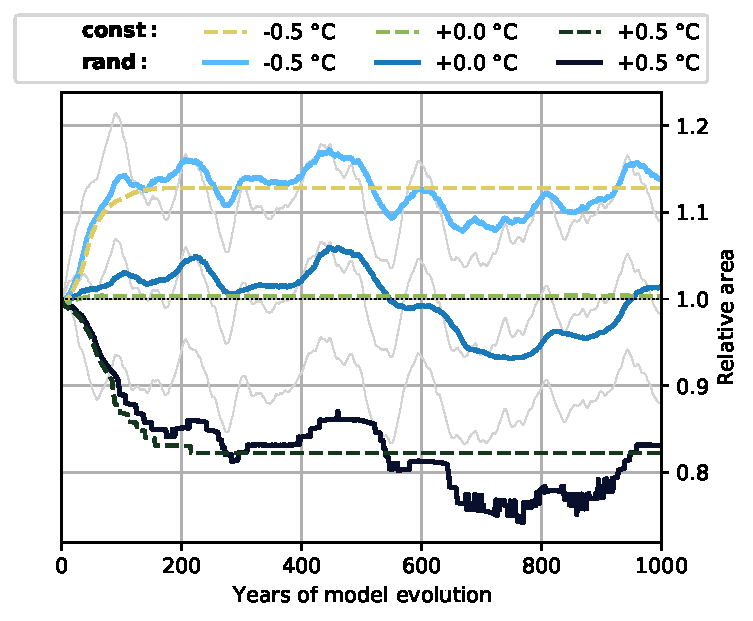
\includegraphics[width=\textwidth]{../plots/final_plots/time_series/single_glaciers/area_norm_fl_Rhonegletscher.pdf}
  \end{subfigure}

  % VAS length
  \begin{subfigure}[b]{0.476\textwidth}
    \caption{\Vas{} model, relative glacier length}
    \label{fig:Rhonegletscher:length_vas}
    \centering
    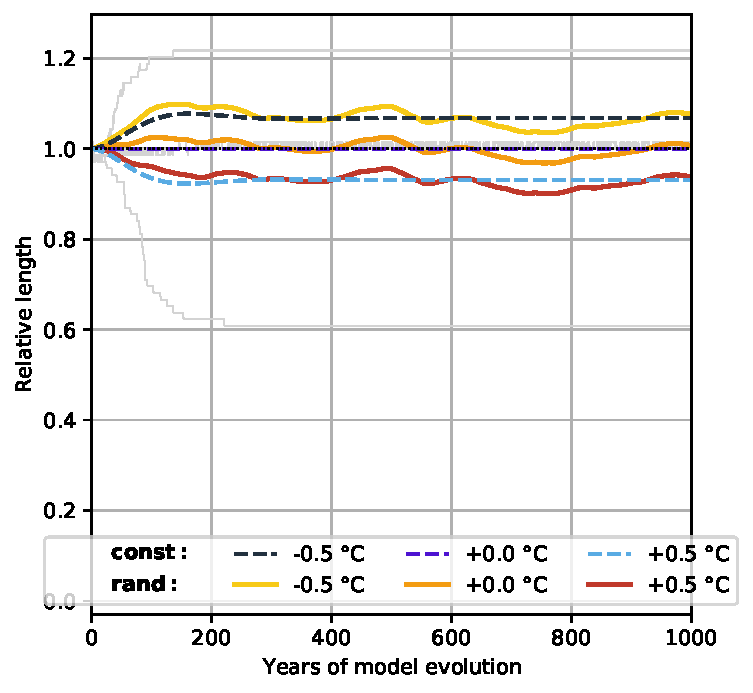
\includegraphics[width=\textwidth]{../plots/final_plots/time_series/single_glaciers/length_norm_vas_Rhonegletscher.pdf}
  \end{subfigure}
  \hfill
  % Flowline length
  \begin{subfigure}[b]{0.476\textwidth}
    \caption{Flowline model, relative glacier length}
    \label{fig:Rhonegletscher:length_fl}
    \centering
    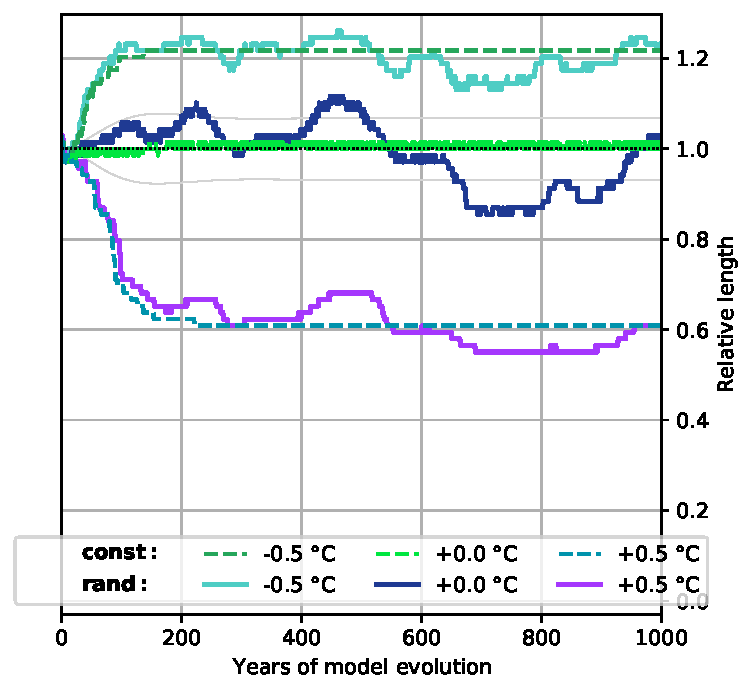
\includegraphics[width=\textwidth]{../plots/final_plots/time_series/single_glaciers/length_norm_fl_Rhonegletscher.pdf}
  \end{subfigure}
  
  \caption{Temporal evolution of ice volume in (\subref{fig:Rhonegletscher:volume_vas}) and (\subref{fig:Rhonegletscher:volume_fl}), surface area in (\subref{fig:Rhonegletscher:area_vas}) and (\subref{fig:Rhonegletscher:area_fl}) and glacier length in (\subref{fig:Rhonegletscher:length_vas}) and (\subref{fig:Rhonegletscher:length_fl}) for \textbf{Rhonegletscher (RGI60-11.01238)}. The shown values area normalized with their respective initial values. The left panels show the result of the \vas{} model, the right panels show the results of the flowline model. Solid lines represent the random climate scenarios, while dashed lines represent the constant climate scenarios. All climate scenarios are based on an equilibrium climate. The applied temperature biases of \SI{-.5}{\celsius}, \SI{0}{\celsius} and \SI{+.5}{\celsius} are color coded, see legend for details. The dotted line indicates the initial volume. The light gray lines represent the volume evolutions of the other model, to facilitate comparisons.}
  \label{fig:Rhonegletscher}
\end{figure}

\chapter{ARMA model order}\label{appendix_B}
\thispagestyle{plain}

\begin{figure}[h!]
  \centering

  % AR
  \begin{subfigure}[b]{0.5\textwidth}
    \caption{Order $p$ for the autoregressive term}
    \label{fig:arma:arp}
    \centering
    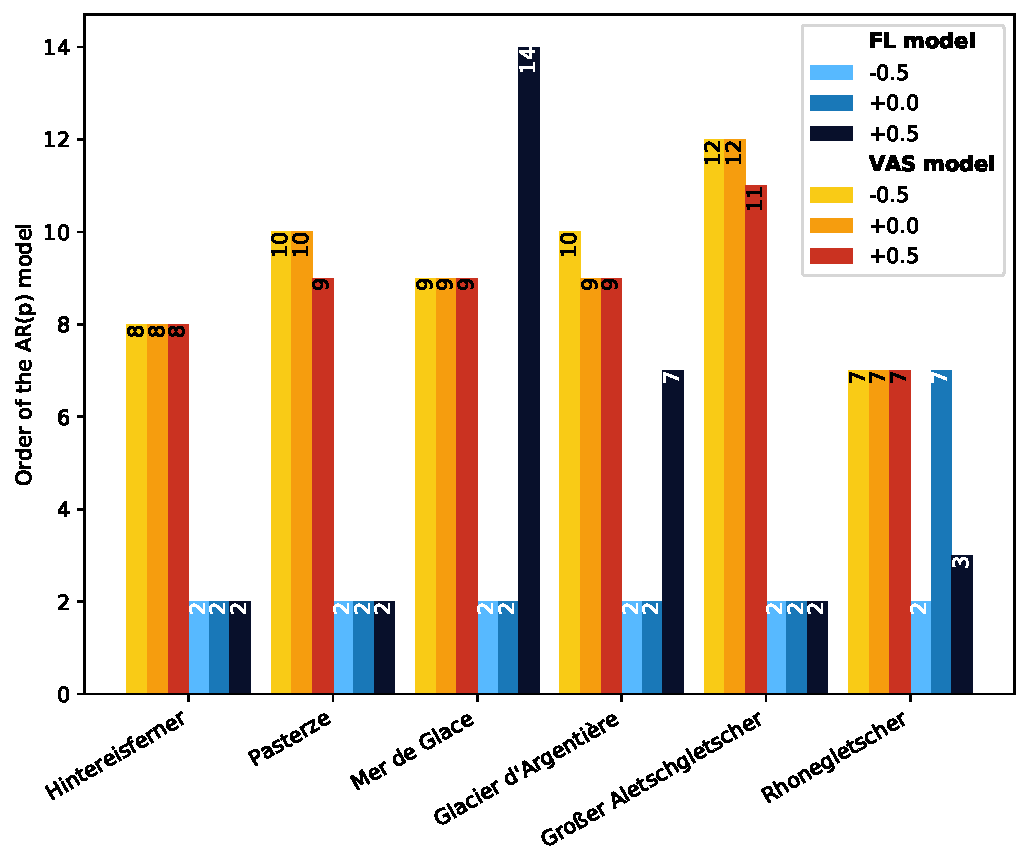
\includegraphics[width=\textwidth]{../plots/final_plots/arma/arp.pdf}
  \end{subfigure}
  \hfill
  % MA
  \begin{subfigure}[b]{0.5\textwidth}
    \caption{Order $q$ for the moving-average term}
    \label{fig:arma:maq}
    \centering
    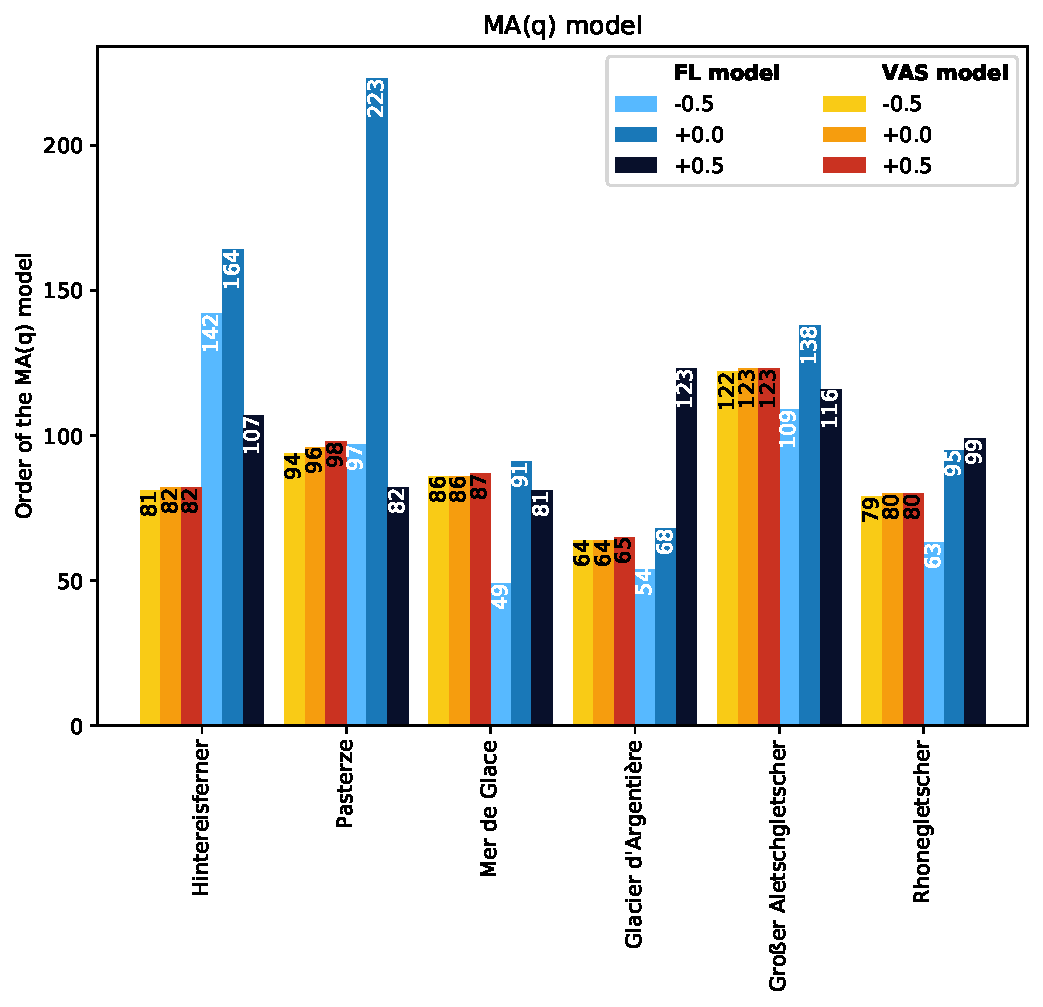
\includegraphics[width=\textwidth]{../plots/final_plots/arma/maq.pdf}
  \end{subfigure}
  
  \caption{Orders $p$ and $q$ for a potential ARMA($p$,$q$) model, estimated from the ACFs and PACFs of the length change signal in response to a white noise climate (see Section~\ref{sub:autocorrelation_function_results})}.
  \label{fig:arma}
\end{figure}

